\documentclass[a4paper]{article}
\usepackage{exercise}
%um nur aufgaben zu zeigen
%\usepackage[noanswer]{exercise} 
\usepackage{../images/preamble}
\usepackage{rotating}
\usetikzlibrary{decorations.pathmorphing}
\usetikzlibrary{decorations.markings}
\usetikzlibrary{arrows}
\usetikzlibrary{shapes.geometric}
\newcommand{\midarrow}{\tikz \draw[-triangle 90] (0,0) -- +(.02,0);}
\usepackage{xcolor}
%\usepackage{draftwatermark}
%\SetWatermarkText{\textsc{Draft 2}}
%\SetWatermarkScale{3}
%\SetWatermarkColor{red!30}

\usepackage[printwatermark]{xwatermark}
%\newsavebox\mybox
%\savebox\mybox{\tikz[color=red,opacity=0.3]\node{\textsc{Entwurf}};}
%\newwatermark*[
%allpages,
%angle=45,
%scale=10,
%xpos=-4cm,
%ypos=4cm
%]{\usebox\mybox}
\pagestyle{fancy}
\fancyhead[L]{
\includegraphics[width=2cm]{../images/logo_scaled.pdf}}
\fancyhead[R]{\textsc{Lösung Aufgabenserie 4}}


\begin{document}
	\vspace*{-1cm}
	\parbox{4cm}{\vspace{-0.2cm}
\includegraphics[width=5cm]{../images/logo_scaled.pdf}}
	\parbox{10.6cm}{\setstretch{2.0} \centering{ \huge \textsf{Aufgabenserie 4 
			}}\\
			Abgabe: 5. Oktober \\ \vspace*{-.5cm} }
		\vspace{0.5cm}

\thispagestyle{empty}
\begin{framed}
	\noindent
	\scriptsize
	Die Aufgaben sollten bis zum \textbf{5. Oktober} bearbeitet werden. Die Lösungen schickt ihr an \href{mailto:physikrolf@gmail.com}{physikrolf@gmail.com}.
	Jede Aufgabe hat eine bestimmte Anzahl an erreichbaren Punkten. Wie viele das sind, müsst ihr raten. Versucht, die Lösungen so genau wie möglich aufzuschreiben. Für besonders schnelle/gute/witzige Lösungen kann es Bonuspunkte geben.\\ Die aktuellen Aufgaben sowie alle alten Aufgabenserien mit Lösungen findet ihr auch auf \url{pankratius.github.io/rolf}. %\\\textit{Zu jeder Aufgabe gibt es jetzt Tipps. Die sollten beim Lösen der Aufgaben helfen.\\ Sollte das so sein macht bitte in euren Lösungen kenntlich, dass bestimmte Schritte von den Tipps und nicht von euch kommen. Darauf gibt es keinen Abzug, es ist nur für uns gut zu wissen.}
\end{framed}

\noindent

\begin{minipage}[b]{0.8\textwidth}
\begin{Exercise}[label = atwood, origin = Aaron Wild, title = Atwoodmaschinen, difficulty = 4]
	Eine Atwoodmaschine besteht im einfachsten Fall aus einer festen Rolle, an der (durch eine masselose Schnur verbunden) zwei Massen $m_1$ und $m_2$ hängen.
	\Question Bestimme für den Fall einer einfachen Atwoodmaschine die Beschleunigung des Systems sowie die Zugkraft im Seil. 
	\ExeText Betrachte jetzt eine unendlichen Atwoodmaschine, bei der alle Massen $m$ betragen.
	\Question Bestimme die Beschleunigung der obersten Masse, für den Fall, dass alle Massen gleichzeitig los gelassen werden.
\end{Exercise}
\end{minipage}
\hfill
\begin{minipage}[t]{0.2\textwidth}
	\centering
		\begin{tikzpicture}
		\draw[thick] (-1,0) -- (1,0);
		\fill[pattern = north east lines] (-1,0) rectangle (1,0.25);
		\draw[thick] (0,0)-- (0,-.5);
		\draw (0,-0.5) circle (0.25);
		\filldraw[black] (0,-0.5) circle (1pt);
		
		\draw (-.25,-0.5) -- (-.25,-1);
		\filldraw[black] (-.25,-1) circle (1.5pt);
		\node at (-.75,-1) {$m$};
		\draw (.25,-0.5)--(.25,-1);
		\draw (.25,-1) circle (0.25);
		\filldraw[black] (.25,-1) circle (1pt);
		\draw (0,-1) -- (0,-1.5);
		\filldraw[black] (0,-1.5) circle (1.5pt);
		\node at (-.5,-1.5) {$m$};
		\draw (.5,-1) -- (.5,-1.5);
		\draw (.5,-1.5) circle (0.25);
		\filldraw[black] (.5,-1.5) circle (1pt);
		\draw (.25,-1.5) -- (.25,-2);
		\filldraw[black] (.25,-2) circle (1.5pt);
		\node at (-.25,-2) {$m$};
		\draw (.75,-1.5) -- (.75,-2);
		\node at (.75,-2.25) {$...$};
		
		
		\end{tikzpicture}
\end{minipage}

\begin{Answer}[ref = atwood]
	\Question Weil die beiden Massestücken der einfachen Atwoodmaschine durch eine Seil fest verbunden sind, müssen sie sich beide mit der Beschleunigung $a$ bewegen, die eine Masse nach oben, und die andere nach unten.\\
	Wir definieren die Bewegungsrichtung der Masse $m_1$ (willkürlich!) als positiv, weswegen die der Masse $m_2$ negativ sein muss. Wenn die Spannkraft im Seil $F_s$ ist, gilt dann für die auf $m_1$ und $m_2$ wirkenden Kräfte
	\begin{subequations}\label{atwood:forces}
		\begin{equation}
			F_s - m_1 g = F_1
		\end{equation}
		\begin{equation}
			m_2 g - F_s = F_2.
		\end{equation}
	\end{subequations}
	In beiden Teilen von \eqref{atwood:forces} gilt nun, dass die Kraft gleich der Masse mal der wirkenden Beschleunigung ist, also $F_1 = m_1 a$ bzw. $F_2 = m_2 a$, sodass \eqref{atwood:forces} ein Gleichungssystem in den beiden Unbekannten $a$ und $F_s$ darstellt, welches einfach gelöst werden kann, um auf
	\begin{subequations}
			\begin{equation}\label{atwood:acc}
			\boxed{	a = \frac{\left(m_2-m_1\right)g}{m_1+m_2}}
			\end{equation}
			\begin{equation}
			\boxed{				T = \frac{2m_1m_2g}{m_1+m_2}.}
			\end{equation}
	\end{subequations}
	zu kommen. \\
	Gleichung \eqref{atwood:acc} macht auch intuitiv Sinn, weil hier für $m_1 = m_2$ für die Beschleunigung $a= 0$ folgt, was heißt, dass sich die Atwoodmaschine bei gleichen Massen nicht aus der stabilen Gleichgewichtslage bewegt (wie wir erwarten würden).
	\Question Dieser Aufgabenteil lässt sich durch eine Skalierungsargumentation für die ersten zwei Rollen lösen. Dazu betrachten wir die Spannung im ersten und zweiten Seil, $F_{S,1}$ bzw. $F_{S,2}$. Die Seilspannung muss sich zwischen dem ersten Massenstück und dem zweiten Seil aufgeteilt haben, sodass $F_{S,2} = \nicefrac{1}{2} F_{S,1}$ gelten muss. \\
	Gleichzeitig können wir analysieren, wie die Wirkung der Gravitations skalieren muss. Dazu überlegen wir uns zuerst, was passieren würden, wenn die Gravitationskraft der Erde um einen Faktor $\nu$ skaliert werden würde. Selbstverständlich würde dann auch die Gravitation um diesen Faktor $\nu$ skaliert werden. Dementsprechend würde aber auch die Spannkraft $F_s$ um einen Faktor $\nu$ skaliert werden, sodass die neue Spannkraft $\nu F_s$ beträgt.\\
	Wenn wir nun die zweite Rolle betrachten, und ihre Beschleunigung $a_2$ nennen, ist die effektiv wirkende Beschleunigung $a_2-g$, weil wir ja noch die Kraft durch die oberste Rolle betrachte müssen.\\
	Weil das \glqq Netzwerk\grqq{} aus Rollen aber unendlich groß sein soll, darf es keinen Unterschied geben, ob man nun die erste oder die zweite Rolle betrachtet. Folglich muss
	\begin{equation}\label{atwood:accsol1}
		\frac{T}{g} = \frac{\nicefrac{T}{2}}{g-a_2}
	\end{equation}
	gelten. Wenn wir jetzt nach $a_2$ umstellen, finden wir, dass $a_2 = \nicefrac{g}{2}$ gelten muss. Weil aber die Beschleunigung der zweiten Masse die gleiche sein muss wie die der ersten Masse, da die beiden ja über ein Seil miteinander verbunden sind, ist auch die Beschleunigung der obersten Masse $\nicefrac{g}{2}$.\\
	%Für den zweiten Lösungsansatz vergleichen wir zuerst den Fall einer Masse $m$, die ohne jegliche Rolle von der Wand hängt, und wieder zwei Massen $m_1$ bzw. $m_2$, die über eine feste Rolle verbunden sind. Die Frage ist nun, wie $m$ gewählt werden muss, damit die Spannkraft $F_{s,m}$ so groß ist, wie die, die in dem System aus $m_1$ und $m_2$ wirkt. 
	%Dazu berechnen wir zuerst wieder die Beschleunigungen bedingt durch Spannkraft und Gravitationskraft. Für den Fall der Ersatzmasse $m$ ist das relativ einfach, und es gilt einfach
	%\begin{equation}\label{key}
	%	
	%\end{equation}
	
\end{Answer}
 
\begin{Exercise}[difficulty = 3, origin = 3. Runde IPhO-Auswahlwettbewerb 2008, title = Bimetallstreifen, label = bms ]
	\hspace{4pt}
	Ein geklebter Bimetallstreifen besteht aus zwei Metallschichten der Dicke $d$, die  Wärmeausdehungskoeffizienten $\alpha_1$ bzw. $\alpha_2$ ($\alpha_2>\alpha_1$) haben. Im Anfgangszustand ist der Streifen gerade. 
	Wie groß ist der Krümmungsradius, wenn der Streifen um $\Delta T$ erwärmt wird? Was passiert im Grenzfall fast gleicher Wärmeausdehungskoeffizienten ($\alpha_2\rightarrow\alpha_1$)?
\end{Exercise}
\begin{Answer}[ref = bms]
	\begin{figure}[h]
		\centering
			\begin{tikzpicture}[scale =1.5]
			\clip(-0.47848681813981486,-1.0992522773586708) rectangle (2.556743060771764,1.7
			191547261822666);
			\draw [shift={(0.,0.)},thick] plot[domain=0.:0.9394498790362418,variable=\t]({1.*1.5*cos(\t r)+0.*1.5*sin(\t r)},{0.*1.5*cos(\t r)+1.*1.5*sin(\t r)});
			\draw [shift={(0.,0.)},thick] plot[domain=0.:0.9394498790362418,variable=\t]({1.*1.*cos(\t r)+0.*1.*sin(\t r)},{0.*1.*cos(\t r)+1.*1.*sin(\t r)});
			\draw [shift={(0.,0.)}] plot[domain=0.:0.9394498790362418,variable=\t]({1.*1.25*cos(\t r)+0.*1.25*sin(\t r)},{0.*1.25*cos(\t r)+1.*1.25*sin(\t r)});
			\draw[thick] (0.5853462909316203,0.800551302621677)-- (0.8851425892165119,1.2105689636734724);
			\draw[thick] (1.,0.)-- (1.5,0.);
				
			\tkzDefPoint(0,0){O}
			\tkzDefPoint(1,0){A}
			\tkzDefPoint(53.83:1){B}
			\tkzMarkAngle[scale = .5](A,O,B)
			\tkzLabelAngle[pos = .55](A,O,B){$\varphi$}
			\tkzDrawPoints(O)
			\tkzDrawSegment[dashed](A,O)
			\tkzDrawSegment[dashed](B,O)
			
			\draw[|-|] (0,-.5) --  (1.25,-.5) node [midway, below] {$R$};
			
			\draw[|-|] (1.25,-0.25) --(1.5,-0.25) node [midway, above] {$d$};
			\end{tikzpicture}
	\end{figure}
	Wir bezeichnen die ursrpüngliche Länge des Bimetallstreifens mit $\ell$. Durch das Erwärmen erhalten wir zwei neue Längen, die gegeben sind durch
	\begin{equation}\label{bms:therm}
		\ell_1 = \ell\left(1+\alpha_1\Delta T\right) ~\mathrm{und}~\ell_2 = \ell\left(1+\alpha_2 \Delta T\right).
	\end{equation}
	Diese Längenänderung führt zu einer kreisförmigen Krümmung des Streifens mit eben dem Krümmungsradius $R$ an der Verbindungsstelle. Den Winkel dieser Krümmung nennen wir $\varphi$. \\
	Damit können wir die neuen Längen jetzt auch als Bogenlängen über dem Winkel $\alpha$ darstellen:
	\begin{equation}\label{bms:arc}
		\ell_1 = \left(R-\frac{d}{2}\right) \varphi ~\mathrm{und}~\ell_2 = \left(R+\frac{d}{2}\right)\varphi.
	\end{equation}
	Die beiden Gleichungen \eqref{bms:therm} und \eqref{bms:arc} stellen nun ein Gleichungssystem da, was man nach $R$ umstellen kann. Wenn man das macht, kommt man auf
	\begin{equation}\label{bms:rsol}
		\boxed{
			R = d\cdot \frac{2+\left(\alpha_1 + \alpha_2\right) \Delta T}{2\left(\alpha_2 - \alpha_1\right)\Delta T}
			}
	\end{equation}
	Im Grenzfall fast gleicher Längenausdehnungskoeffizienten sollte es nicht zu einer Krümmung kommen, weil sich ja beide Streifen gleich stark ausdehnen. Dementsprechend sollte der Krümmungsradius gegen unendlich gehen.\\
	Das sehen wir auch an dem dimensionslosen, zweiten Faktor in Gleichung \eqref{bms:rsol}. Im Fall $\alpha_2\rightarrow \alpha_1$ kommt der Nenner des Bruchs immer näher an null, sodass der Krümmungsradius ohne jede Grenze steigt, also keine Krümmung vorliegt.
\end{Answer}
\begin{Exercise}[label = trinity, origin = Aaron Wild, title = {Project Trinity}, difficulty = 3]
	\hspace{0.02pt}
	Die Ausbreitung einer halbkreisförmigen Schockwelle hängt von der Energie $E$ der Explosion sowie der Dichte der Luft $\rho$ ab.
	\Question Bestimme eine Gleichung, die den Radius $R$ der Schockwelle als Funktion der Zeit $t$ nach der Explosion angibt.
	\ExeText Die folgenden Bilder zeigen die Schockwelle nach dem ersten Atombombentest der USA 1945, \textit{Project Trinity}:
		\begin{figure}[h]
		\begin{subfigure}[b]{0.5\textwidth}
			\centering
			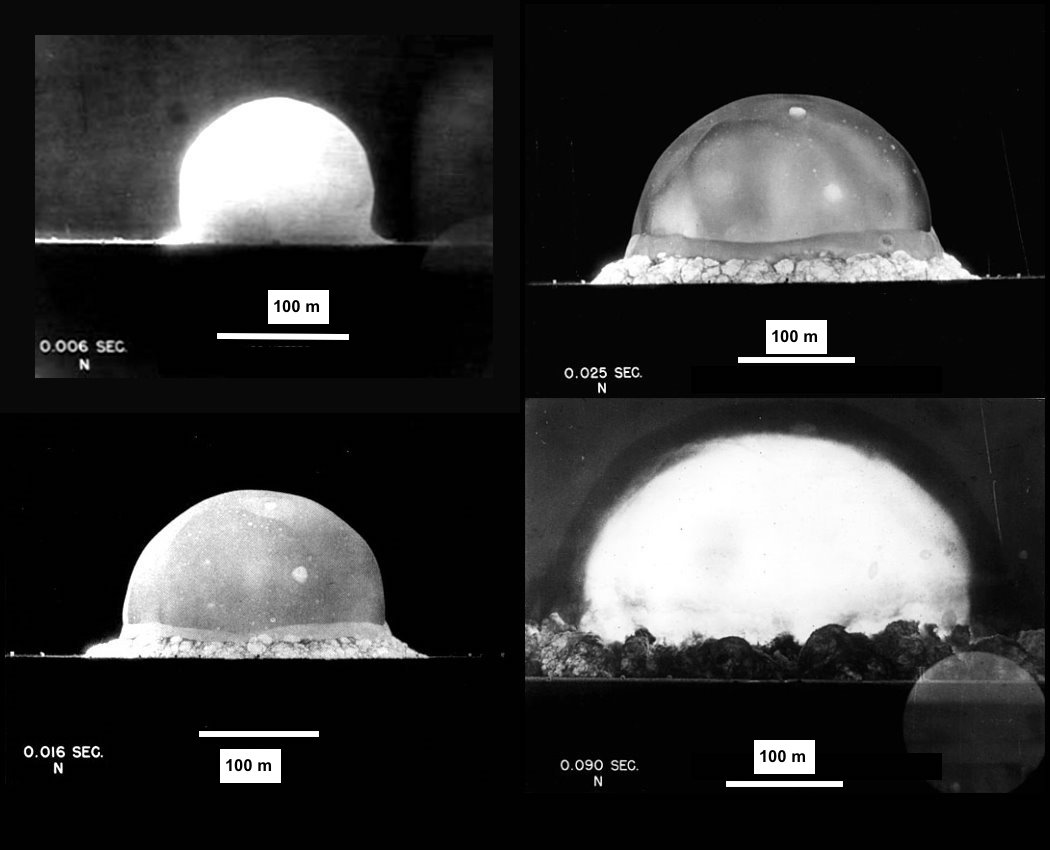
\includegraphics[scale = 0.2]{../tasks/selfmade/trinityim.jpeg}
		\end{subfigure}
		\begin{subfigure}[b]{0.5\textwidth}
			\centering
			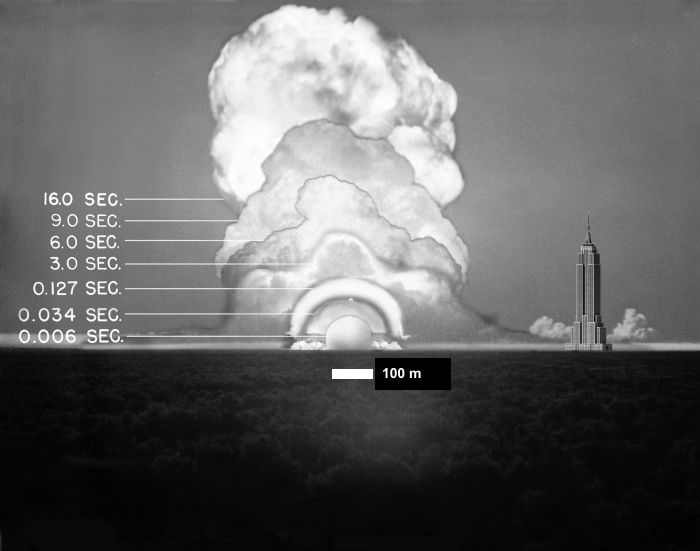
\includegraphics[scale = 0.25]{../tasks/selfmade/trinityim2.png}
		\end{subfigure}
		\caption{Massstabsgerechte Abbildung einer Schockwelle nach der Detonation}
		\label{fig:trinityim}
		\end{figure}
	\Question Unterstützen diese Bilder dein Ergebnis aus 1.?
\end{Exercise}
\begin{Answer}[ref  = trinity]
	\Question Um den Radius als Funktion der Zeit darstellen zu können, reicht es, wenn wir uns fragen, wie man die gegebenen Größen ($E$, $\rho$  und $t$) miteinander multiplizieren muss, damit am Ende eine Größe mit der Einheit eines Radius, also Meter, da steht.\\
	Dazu ist es sinnvoll, sich von den konkreten Einheitensystemen zu lösen, und mit sog. Dimensionen zu rechnen. Diese sind in unserem Fall die Dimensionen der Zeit $T$, der Masse $M$ und der Strecke $M$. Der Vorteil von Dimensionen ist, dass sie uns von willkürlichen Einheiten befreien. Es ist also egal, ob wir eine Masse in Pfund oder Kilogramm angeben, ihre Dimension bleibt immmer die der Masse, $M$. Bei einem Volumen ist es egal, ob wir es in $m^3$ oder in Unzen angeben, die Dimension bleibt immer $L^3$.\\
	Die Dimension der Zeit zu finden ist doch eher einfach, es ist nämlich nur $T$. Für die der Dichte können wir uns die Definitionsgleichung anschauen, $\rho = \nicefrac{m}{V}$. $m$ ist eine Masse, hat also als Dimension $M$; $V$ ist ein Volumen, hat also als Dimension eine Länge im Kubik, $L^3$. Die Energie ist ein wenig schwieriger. Wir wissen aber, dass die Energie definiert ist als Kraft mal Weg ($ E = Fs$), und die Kraft wiederum als Masse mal Beschleunigung ($F = m a$), und die Beschleunigung wiederum ist Geschwindigkeitsänderung pro Zeit ($a = \nicefrac{v}{t}$), und die Geschwindigkeit selber ist Wegänderung pro Zeit ($v=\nicefrac{s}{t}$.) Ab jetzt wird es sinnvoll, sich eine Notation für die Dimension einer Größe auszudenken. Das macht man, indem man die Größe in eckige Klammern packt, also $\left[t\right] = T$ und so weiter. Für die Energie kommen wir, wenn wir all das einfach zusammen packen, auf $\left[E\right] = L^2 \cdot M\cdot T^{-2}$.\\
	Jetzt können wir anfangen, die Aufgabe zu lösen. Dazu können wir zuerst einmal schauen, was passiert, wenn wir $E$, $t$ und $\rho$ einfach ohne nachzudenken brachial zusammen multiplizieren. Nennen wir diese Größe $\nu = Et\rho$. Dann ist deren Dimension gegeben durch
	\begin{equation}\label{trinity:wrongsol}
		\left[\nu \right] = \left[E\right]\cdot \left[t\right]\cdot \left[\rho\right] = L^2\cdot M \cdot T^{-2}\cdot T \cdot M \cdot L^{-3} = L^{-1}\cdot M^2 \cdot T^{-1}.
	\end{equation}
	Wir sehen, dass einfach multiplizieren nicht klappt (Wir erwarten ja $\left[\nu\right] = \left[R\right] = L$)!\\
	Also müssen wir uns einen allgemeineren Ansatz überlegen. Der Ansatz, der am Allgemeinsten ist, ist einfach, irgendwelche Potenzen für die drei Größen anzunehmen ($\alpha$, $\beta$ und $\gamma$), und dann zu schauen, wie man diese wählen muss, damit die Dimensionen aufgehen\footnote[2]{Ab jetzt werden Potenzgesetze wirklich hilfreich!}. In diesem Fall also
	\begin{equation}\label{trinity:dim1}
		\left[R\right] = L \overset{!}{=} \left[E\right]^\alpha\cdot\left[t\right]^\beta\cdot\left[\rho\right]^\gamma = L^{2\alpha} \cdot M^\alpha\cdot T^{-2\alpha}\cdot T^\beta\cdot M^\gamma \cdot L^{-3\gamma} = L^{2\alpha-3\gamma}\cdot M^{\alpha + \gamma} \cdot T^{-2\alpha + \beta}.
	\end{equation}
	Wir wollen jetzt $\alpha$, $\beta$ und $\gamma$ so wählen, dass die Dimension stimmt, also links und rechts des Gleichheitszeichens wirklich auch die gleichen Sachen stehen. Es sollen die drei Exponeten also so gewählt werden, dass $L$ den Exponenten 1 hat, und $M$ und $T$ jeweils null. Daraus können wir ein Gleichungssystem schreiben
	\begin{subequations}\label{trinity:soe}
		\begin{equation}\label{trinity:a1}
			2\alpha - 3\gamma  = 1
		\end{equation}
		\begin{equation}\label{trinity:a2}
			\alpha + \gamma = 0
		\end{equation}
		\begin{equation}\label{trinity:b1}
			-2\alpha + \beta = 0.
		\end{equation}
	\end{subequations}
	Das kann man einfach lösen\footnote[3]{Dazu stellt man am Besten \eqref{trinity:a2} nach $\gamma$ um, $-\alpha = \gamma$, und setzt dann in \eqref{trinity:a1} ein. Da kommt man auf $2\alpha + 3\alpha = 1 \Rightarrow 5\alpha = 1 \Rightarrow \alpha = \nicefrac{1}{5}$. Damit hat man dann sofort $\gamma  = -\alpha = -\nicefrac{1}{5}$ und $\beta = -2\alpha = -\nicefrac{2}{5}$ (über \eqref{trinity:b1})}, und kommt auf $\alpha = \nicefrac{1}{5}$, $\beta = \nicefrac{2}{5}$ und $\gamma = -\nicefrac{1}{5}$, womit $R\left(t\right)$ also gegeben ist durch
	\begin{equation}\label{trinity:rt}
		R\left(t\right) = E^{\nicefrac{1}{5}}\cdot t^{\nicefrac{2}{5}} \cdot \rho^{-\nicefrac{1}{5}} = \sqrt[5]{\frac{Et^2}{\rho}}.
	\end{equation}
	Das Ergebnis ist aber noch nicht vollständig! Was wir durch die Dimensionsanalyse nämlich nicht feststellen können, ist, ob in dem Produkt \eqref{trinity:rt} nicht noch irgendeine Zahl steht (also z.B. $\nicefrac{\pi}{4}$, $30000$ oder $e^{\sqrt{2}}$. ), weil sich dadurch ja die Dimension des Ergebnis nicht ändert. Um die allgemein mögliche Lösung zu finden, müssen wir also schreiben
		\begin{equation}\label{trinity:rtc}
			\boxed{
				R\left(t\right) = c\cdot \sqrt[5]{\frac{Et^2}{\rho}},
				}
		\end{equation}
		wobei $c$ eben diese Konstante ist. Die könenn wir durch die Dimensionsanalyse aber nicht abschätzen (wie auch?). Das stattdessen kann man hier entweder auf experimentelle Daten zurückgreifen, oder aber weitere theoretische Analysen betreiben.
	\Question Da die Bilder massstabsgerecht sind, können wir daraus $R\left(t\right)$ messen, indem wir ein Lineal nehmen (dabei ist es sinnvoll, nach $t=0.127~\mathrm{s}$) aufzuhören. Es ergeben sich folgende Werte
	\begin{table}[h]
		\centering
	\begin{tabular}{|c|c|}
		\hline
	$t/\mathrm{s}$	& $R/\mathrm{m}$ \\ 
		\hline \hline 
	0.006	& 95.0 \\ 
		\hline 
	0.016	& 114.0 \\ 
		\hline 
	0.025	& 124.0 \\ 
		\hline 
	0.034	& 143.0 \\ 
		\hline 
	0.09	&  175.0\\ 
		\hline 
	0.127	&  179.0\\ 
		\hline 
	\end{tabular} 
	\caption{Messwerte aus den Abbildungen}
	\label{trinity:t1}
\end{table}
	Wir können jetzt schauen, ob diese Messwerte tatsächlich dem Zusammenhang $R\propto \sqrt[5]{t^2}$ entsprechen, wie wir ihn aus \eqref{trinity:rtc} erwarten würden.\\
	Dazu können wir einen Graphen zeichnen. Wenn wir uns aber einfach nur den Graphen $R\left(t\right)$ anschauen, können wir da nicht viel erkennen.
	\begin{figure}[h]
\centering
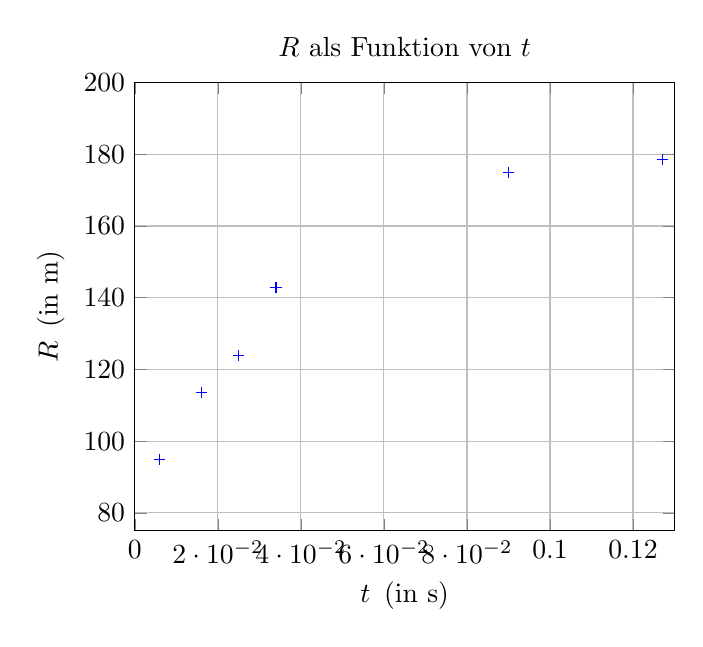
\begin{tikzpicture}
	\begin{axis}[xmin = 0, xmax = 0.13, ymin = 75, ymax = 200, grid = major, xlabel = {$t~\left(\mathrm{in~s}\right)$}, ylabel = $R~\left(\mathrm{in~m}\right)$, title ={ $R$ als Funktion von $t$} ]
%x labels  = {0,0.02,0.04,0.08,0.10,0.12}
\addplot[blue, only marks, mark = +] coordinates
{(0.006, 95.)  (0.025, 123.81) (0.016, 113.636) (0.09, 
	175.) (0.034, 142.857) (0.127, 178.571)
	};

	\end{axis}
\end{tikzpicture}
\end{figure}
	 Viel besser wird es, wenn wir $R^5\left(\sqrt{t}\right)$ zeichnen. Das sollte dann nämlich einfach eine lineare Funktion sein. Danach sieht es auch aus.
	 \begin{figure}[h]
\centering
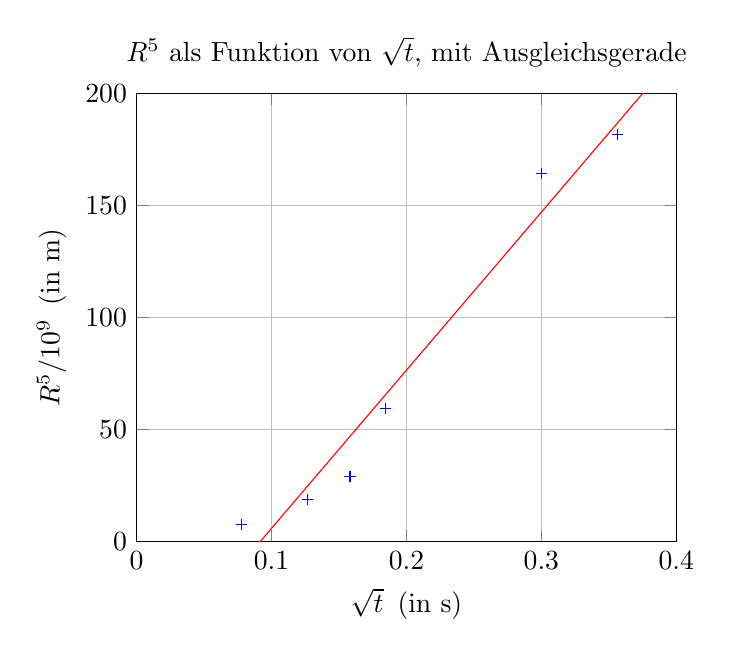
\begin{tikzpicture}
	\begin{axis}[xmin = 0, xmax = 0.4, ymin = 0, ymax = 200, grid = major, xlabel = {$\sqrt{t}~\left(\mathrm{in~s}\right)$}, ylabel = $R^5/10^{9}~\left(\mathrm{in~m}\right)$, title ={ $R^5$ als Funktion von $\sqrt{t}$, mit Ausgleichsgerade} ]

\addplot[blue, only marks, mark = +] coordinates
{(0.0774597, 7.73781) (0.158114, 29.0918) (0.126491, 18.949) (0.3, 
		164.131) (0.184391, 59.499) (0.356371, 181.577)};

\addplot[red] {-64.532+705.153*x};

	\end{axis}
\end{tikzpicture}
\end{figure}
	 Es scheint also, als sei unser Ergebnis aus 1. im Einklang mit diesen Messwerten. Schön ist, dass wir dafür $c$ gar nicht kennen müssen!
	 Eigentlich muss man hier noch eine Fehleranalyse machen!
\end{Answer}



\end{document}